
\section*{Problema P6.25}

\renewcommand*\thesection{6.25}
\numberwithin{equation}{section}

\begin{center}
    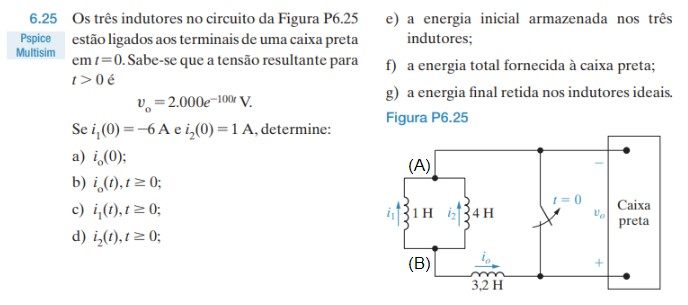
\includegraphics[scale=1.0]{P6.25.jpg}
\end{center}

\subsection*{(a)}

Aplicando análise nodal no nó essencial (B), temos

\[ i_0(t) + i_1(t) + i_2(t) = 0 \logo i_0(t) = - i_1(t) - i_2(t)  \]

Substituindo no instante $t=0$,

\[ i_0(0) = -(-6) - 1   \]

\[ \boxed{i_0(0) = 5 \un{A}}  \]

\subsection*{(b)}

Reduzindo os três indutores da figura via redução série-paralelo, temos um indutor equivalente $L_{eq}$ dado por 

\[ L_{eq} = (1\un{H} \;//\; 4\un{H}) + 3.2\un{H}  \]

\[ L_{eq} = 4.0\un{H}  \]

Assim, usando a expressão da corrente no indutor

\begin{equation}\label{eq:6.25.1}
    i_0(t) = i_0(0) + \frac{1}{L} \int_{t_i}^{t_f} v_L(t) \,dt
\end{equation}

Note que no sentido em que $i_o(t)$ está definida na figura, temos, via análise de malhas,

\[+v_o(t) + v_{L_{eq}}(t) = 0  \logo  v_{L_{eq}}(t) = - v_o(t) \]

Assim, temos que \eqref{eq:6.25.1} deve ter o sinal ajustado para atender a convenção passiva definida acima, ficando

\begin{equation}\label{eq:6.25.2}
    i_0(t) = i_0(0) - \frac{1}{L} \int_{t_i}^{t_f} v_0(t) \,dt
\end{equation}

Substituindo os valores do enunciado e resultado do item (a) em \eqref{eq:6.25.2}, temos

\[ i_0(t) = 5 - \frac{1}{4}\int_{0}^{t} 2000e^{-100t} \,dt  \]

\[ i_0(t) = 5 - 2000\frac{1}{4}\frac{1}{-100}\left[e^{-100t} - e^{0}\right]  \]

\[ i_0(t) = 5 + 5\left[e^{-100t} - 1\right]  \]

\[ \boxed{i_0(t) = 5e^{-100t} \quad ,  \quad t \geq 0}  \]

\subsection*{(c)}

Retornando ao circuito original, temos que a queda de tensão no indutor $L_0 = 3.2\un{H}$ é dada por

\[ v_{L_0}(t) = L_0\diff{i_0}{t} \]

Substuindo o resultado encontrado no item (b), temos

\[ v_{L_0}(t) = 3.2(-500e^{-100t}) \un{V} = -1600e^{-100t} \un{V} \]

Assim, aplicamos análise de malhas para determinar a queda de tensão indutor $L_1 = 1 \un{H}$, assumindo
$i_0(t)$ como a corrente de malha no sentido que ela foi definida na figura.

\[ v_o(t) + v_{L_0}(t) - v_{L_1}(t) = 0 \]

\begin{equation}\label{eq:6.25.3}
    v_{L_1}(t) = v_o(t) + v_{L_0}(t)
\end{equation}

Substituindo os resultados encontrados em \eqref{eq:6.25.3}, temos

\[ v_{L_1}(t) = 2000e^{-100t} - 1600e^{-100t} \]

\[ v_{L_1}(t) = 400e^{-100t} \un{V} \]

Assim, novamente usando \eqref{eq:6.25.1}, temos a corrente $i_1(t)$ dada por 

\[ i_1(t) = -6 + \frac{1}{1}\int_{0}^{t} 400e^{-100t} \,dt  \]

\[ i_1(t) = -6 + \frac{1}{-100}400 \left[e^{-100t} - e^0\right]  \]

\[ \boxed{i_1(t) = -2 -4 e^{-100t} \un{A} \quad ,  \quad t \geq 0}  \]

\subsection*{(d)}

Usando a análise nodal do item (a), temos

\[ i_2(t) = - i_0(t) - i_1(t)  \]

Substituindo os valores encontrados nos itens anteriores,

\[ i_2(t) = - (5e^{-100t}) - (-2 -4 e^{-100t}) \]

\[ \boxed{i_2(t) = 2 - e^{-100t} \un{A} \quad ,  \quad t \geq 0}  \]

\subsection*{(e)}

Sabemos que a energia armazena em um indutor é dada por 

\begin{equation}\label{eq:6.25.4}
    E(t) = \frac{1}{2}L\left[i(t)\right]^2
\end{equation}

Em $t=0$ usamos os valores de $i(0)$ para cada um dos indutores, obtendo

\[ E_0(0) = 40 \un{J} \quad , \quad E_1(0) = 18 \un{J} \quad , \quad E_2(0) = 2 \un{J}   \]

A energia total armazenada em $t=0$ é, portanto, 

\[ E_T(0) = E_0(0) + E_1(0) + E_2(0)  \]

\[ \boxed{E_T(0) = 60 \un{J}}  \]

\subsection*{(f)}

Usando o circuito equivalente com $L_{eq} = 4\un{H}$ e \eqref{eq:6.25.4} em $t=0$, temos

\[ E_{ent}(0) = \frac{1}{2}L_{eq}[i_0(0)]^2  \]

\[ E_{ent}(0) = \frac{1}{2}4[5]^2  \]

\[ \boxed{E_{ent}(0) = 50 \un{J}}  \]

\subsection*{(g)}

A energia retida $E_R(t)$ em $t=0$ é dada pela diferença entre a energia inicialmente armazenada e a entregue. Assim,    

\[ E_{R}(0) = E_T(0) - E_{ent}(0)  \]

\[ E_{R}(0) = 60\un{J} - 50\un{J}  \]

\[ \boxed{E_{R}(0) = 10\un{J}}  \]

